\section{A Running Example: DrawableDeck}~\label{sec:overview}
This section illustrates the features of our \MIM{} model for
resolving unintentional method conflicts. As mentioned before, such a
case arises when two inherited methods happen to have the same
signature, but with different semantics and functionality. This
situation is troublesome to programmers that use multiple
inheritance. Below we illustrate with a running example called
\lstinline|DrawableDeck|, which models a drawable deck of cards. 
Note that we use Java-like syntax
throughout the paper, and all types are defined with the keyword
``\lstinline|interface|''. The concept is closely related to Java 8
interfaces with default methods~\cite{}, and traits. For simplicity, an interface in our model has
the following characteristics:
\begin{itemize}
	\item It allows multiple inheritance.
	\item Every method represents a behaviour and requires a body for its implementation (like Java 8 default methods). There are no abstract methods.
	\item It can be directly instantiated by the \lstinline|new| keyword.
\end{itemize}
Furthermore for simplicity, our formalization does not model state at
this stage. %%, but that should not block our discussions below.
\bruno{I think there are two important things being discussed in this
  section:
1) Hierarchical dispatch: which allows methods calls to be correctly 
dispatched based on a combination of static and dynamic type
information; and
2) Traingle Inheritance: i.e. allowing multiple method implementations 
to coexist in the same class based on the superclass hierarchy. 

The text in this section is good, but it could emphasize better those 
two aspects. I think the text starts off with point 2) (the two draw
methods), then in between the discussion moves to hierarchical
dispatching. Later it returns to point 2. 
}

\subsection{Problem 1: Unintentional Method Conflicts}
Suppose that two components \lstinline|Deck| and \lstinline|Drawable| 
have been developed in a system.  \lstinline|Deck| represents a deck
of cards, and defines \lstinline|draw()| for drawing a card from the
deck.  \lstinline|Drawable| is an interface for graphics that
can be drawn, and also includes a method called \lstinline|draw()| for
visual display. For illustration, the implementation of
\lstinline|draw()| in \lstinline|Drawable| only creates a blank canvas
on the screen, and later some instances (\lstinline|Circle|,
\lstinline|Square|, or others) that extend \lstinline|Drawable| may
define their own \lstinline|drawObject()| methods and invoke
\lstinline|draw()|.

\vspace{3pt}\begin{lstlisting}
interface Deck {
  void draw() { // draws a card from the Deck
    Stack<Card> cards = this.getStack();
    if (!cards.isEmpty()) {
      Card card = cards.pop();
      ...
    }
  }
}

interface Drawable {
  void draw() { // draws something on the screen
    JFrame frame = new JFrame("Canvas");
    frame.setVisible(true);
    ...
  }
}
\end{lstlisting}\vspace{3pt}
\bruno{Space is probably going to be a problem, so you may have to
  consider putting code side-by-side to maximize space usage.}
Note that both methods have \lstinline|void| return type (we will not formalize
\lstinline|void| in our calculus afterwards; here is only for illustration). In \lstinline|Deck|, \lstinline|draw()| tries to get the cards as a stack, pops
out the top card, and so on. While in \lstinline|Drawable|, \lstinline|draw()|
creates a blank canvas using \lstinline|JFrame|. Now, a programmer is designing a
card game with GUI. He may want to draw a deck on the screen, so he defines a drawable
deck using multiple inheritance:

\vspace{3pt}\begin{lstlisting}
interface DrawableDeck extends Drawable, Deck {...} 
\end{lstlisting}\vspace{3pt}
The point of using multiple inheritance is surely for composing the features from various 
components, and to achieve code reuse. Multiple inheritance is supported by many mainstream OO
languages. Nevertheless at this point, \lstinline|DrawableDeck| has to throw a compile
error, since the two \lstinline|draw()| methods cause a conflict, though accidentally.

\subsection{Potential Fixes}

For that problem, there are several workarounds. We go over some of
the main ones next.

\paragraph{I. Delegation.} As an alternative to multiple inheritance,
delegation can be used by introducing two fields with
\lstinline|Drawable| type and \lstinline|Deck| type,
respectively. This avoids method conflicts. Nevertheless, it is known
that using delegation makes it hard to correctly maintain
self-references \haoyuan{?} in an extensible system [], and also
introduces a lot of boilerplate code.

\paragraph{II. Creating a \lstinline|draw()| method in \lstinline|DrawableDeck|, which explicitly overrides the old ones.}
This is a non-solution. It does not make any sense to override both methods with totally different functionalities, as old
methods have to be hidden.

\paragraph{III. Refactor Drawable and/or Deck to rename the methods.} If
the code for \lstinline|Drawable| or \lstinline|Deck| are available
then it may be possible to rename one of the \lstinline|draw|
methods. However this approach is non-modular, as it requires 
modifying existing code, and may not be possible if code is unavailable.

%\paragraph{III. Choosing one of them as the default method, like Mixins.} The mixin model can be applied to choose a
%default one based on linearisation. Similarly, we want to preserve both features, rather than keeping only one of them.

\paragraph{IV. Method exclusion/renaming in traits.} Some trait models
support method exclusion/renaming. Those features
provided can eliminate conflicts, although most
programming languages do not support them. In a traditional OO system,
they can break the subtyping. Moreover, in
contrast with exclusion, renaming can indeed preserve both conflicted
behaviours, however, it is cumbersome in practice, as introducing new
names can affect other code blocks.

\paragraph{V. Static dispatch.}
What we really expect from the language is keeping both methods
without renaming, and the type checker does not complain. 
But we need to find an approach to \emph{disambiguate on method
calls statically}.
\bruno{Perhaps show the solution in MIM here (i.e Section 2.4), and then move to problem
2 (which is being discussed next with shuffleAndDraw)}

Certainly the compiler can ignore the conflict when
\lstinline|DrawableDeck| is declared, but once an object of
\lstinline|DrawableDeck| is created, a method call for
\lstinline|draw()| on that object would be ambiguous. Nonetheless, we can adopt static dispatch for
disambiguating. Some languages like C++ use qualified names in that
way:

\vspace{3pt}\begin{lstlisting}
void func(Drawable obj) {
  obj.draw();
}

DrawableDeck d = new DrawableDeck();
d.Drawable::draw();       // calling draw() in Drawable
((Drawable) d).draw(); // calling draw() in Drawable
func(d);                 // calling draw() in Drawable
\end{lstlisting}\vspace{3pt}
Static dispatch in C++ finds out and invokes the most specific method ``by need''.

\subsection{Problem 2: Dynamic Dispatch for Code Reuse}
\begin{figure*}[t]
\centering
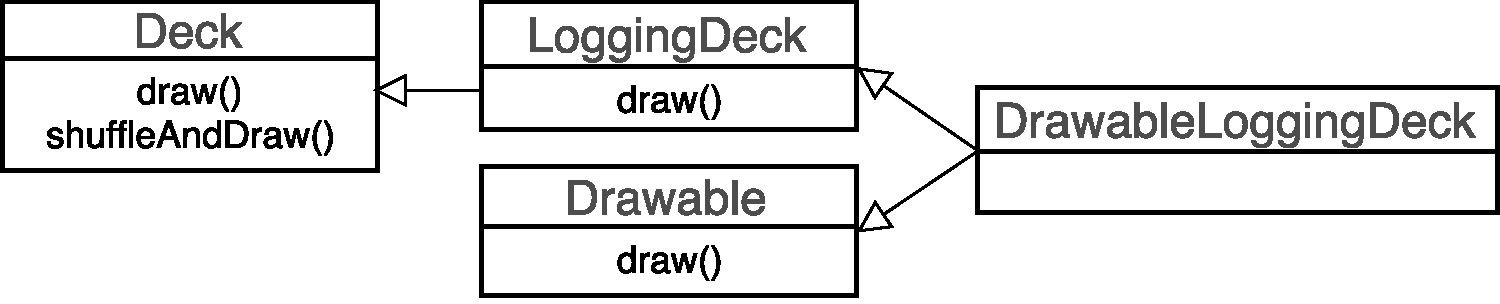
\includegraphics[height=2cm]{pics/DrawableLoggingDeck.pdf}
\caption{DrawableLoggingDeck UML}\label{fig:drawableloggingdeck}
\end{figure*}

On the other hand, we also need dynamic dispatch as it is essential and widely used in object-oriented programming.
C++ has the flexibility for choosing either way of dispatch by the \kwvirtual{} keyword.
Unfortunately, this approach is still unsatisfactory regarding code reuse. For instance in Figure~\ref{fig:drawableloggingdeck}, 
we redefine \lstinline|Deck| to support
both \lstinline|draw()| and another operation called \lstinline|shuffleAndDraw()|:
\vspace{3pt}\begin{lstlisting}
interface Deck {
  void draw() {...}
  void shuffleAndDraw() {
    shuffle();
    draw();
  }
  ...
}
\end{lstlisting}\vspace{3pt}
\lstinline|shuffleAndDraw()| is a representative method that invokes \lstinline|draw()| in its definition. In principle, we want
that invocation to use dynamic dispatch, because a programmer may define a subtype of \lstinline|Deck|, and override \lstinline|draw()|:
\vspace{3pt}\begin{lstlisting}
interface LoggingDeck {
  void draw() { // overriding
    Stack<Card> cards = this.getStack();
    if (!cards.isEmpty()) {
      Card card = cards.pop();
      println("The card is: " + card.toString());
      ...
    } else {
      println("Empty deck.");
    }
  }
}
\end{lstlisting}\vspace{3pt}
Usually we want to reuse the code of \lstinline|shuffleAndDraw()| during inheritance, hence dynamic dispatch is necessary, otherwise
programmers have to override all the other methods that invoke \lstinline|draw()|. However, as seen before, dynamic dispatch can cause
ambiguity if we have:
\vspace{3pt}\begin{lstlisting}
interface DrawableLoggingDeck extends Drawable, LoggingDeck {...}

DrawableLoggingDeck d = new DrawableLoggingDeck();
d.shuffleAndDraw(); // ambiguous draw()
\end{lstlisting}\vspace{3pt}
Since the dynamic type of the receiver is \lstinline|DrawableLoggingDeck|, calling \lstinline|shuffleAndDraw()| triggers the ambiguity. When \lstinline|shuffleAndDraw()| invokes \lstinline|draw()|, what we really want is \lstinline|LoggingDeck.draw()|, yet
neither static dispatch nor dynamic dispatch in languages like C++ does so.
 Therefore, we need to find another algorithm for method resolution.

\subsection{Solution in \MIM: \dispatchnamecaptical}\label{subsec:solutionmim}
The \MIM{} model uses \dispatchnameit{} for method lookup. A qualified
method invocation, for instance, \lstinline|e.I::m()|, is read as
``finding the most specific method \lstinline|m| along the path
\lstinline|I|''. The meaning of ``along the path \lstinline|I|'' is
that, if the result of \dispatch{} is \lstinline|J.m()| for some \lstinline|J|, then such a \lstinline|J| must be a super type of \lstinline|e|'s dynamic type, and \lstinline|J| has a subtyping relation with \lstinline|I| (either \lstinline|J <: I| or \lstinline|J >: I|). Intuitively, the most specific \lstinline|m()| must be from branch \lstinline|I|, but it can be an overridden version after \lstinline|I| because of dynamic dispatch. The formal definition will be introduced later. On the other hand, \lstinline|e.m()| where \lstinline|e| has static type \lstinline|I|, simply behaves the same as \lstinline|e.I::m()| in our model. It is just like the difference between implicit and explicit casts.

Such a dispatch algorithm make uses of both the static type and the dynamic type of the receiver. Intuitively, the static type specifies one branch of the method to avoid ambiguity, and the dynamic type finds the latest version on that branch. It may still introduce ambiguity when there are multiple paths from the static type to the dynamic type, and those paths cause conflicts. To prevent this, we disallow this kind of conflict to ensure unambiguity. That is to say, we do not allow two methods to override a same base method when they cause conflicts. This is natural, as they are just two versions of the same operation, hence it is no longer an ``unintentional'' conflict in that way.

With the old example, the code below meets our expectation:
\vspace{3pt}\begin{lstlisting}
interface Deck {
  void draw() {...}
  void shuffleAndDraw() {
    this.Deck::shuffle();
    this.Deck::draw();
  }
  ...
}
\end{lstlisting}\vspace{3pt}
It guarantees that \lstinline|shuffleAndDraw()| calls \lstinline|shuffle()| and \lstinline|draw()| from its own branch, so that the namesakes
from other branches will not cause conflicts. Now \lstinline|d.shuffleAndDraw()| is no longer ambiguous.

Actually in \MIM{}, we can still write ``\lstinline|shuffle();|'' and ``\lstinline|draw();|'',
because the compiler is able to know that the receiver ``\lstinline|this|'' exactly has static type \lstinline|Deck|, hence hierarchical dispatch eliminates ambiguity.

\subsection{Partial Overrides in \MIM	}\label{subsec:partialoverrides}

Method overriding is commonly supported by many OO languages as a kind of polymorphism.
We have seen that \MIM{} is able to preserve several conflicted branches simultaneously and let them coexist.
In that case, a traditional method overriding, like one in Java, will override all the inherited methods, and hence
hide all those conflicted branches. Besides, \MIM{} also allows partial overrides to offer independent extensibility.
A partial override will specify one of the branches, and only refine the method from that branch. It ensures that
other branches are not affected.

For example, we define an interface \lstinline|DrawableLoggingDeck2|, and in its definition we refine the \lstinline|draw()| from \lstinline|Drawable()| by setting
the canvas invisible:
\vspace{3pt}\begin{lstlisting}
interface DrawableLoggingDeck2 extends DrawableLoggingDeck {
  void draw() override Drawable {
    JFrame frame = new JFrame("Canvas");
    frame.setVisible(false);
    ...
  }
}
\end{lstlisting}\vspace{3pt}
Here the partial override specifies \lstinline|Drawable| to be refined. The use of it ensures that both branches of \lstinline|draw()| are preserved. At the same time, we should notice that the methods we present in previous examples are called ``original methods'', and they are actually created by ``total overrides'', rather than partial overrides. Some client code is shown below: \haoyuan{which words should we use instead of "total overrides"?}
\vspace{3pt}\begin{lstlisting}
DrawableLoggingDeck2 d2 = new DrawableLoggingDeck2();
d2.Drawable::draw(); // calling draw() in DrawableLoggingDeck2
d2.Deck::draw();       // calling draw() in LoggingDeck
\end{lstlisting}\vspace{3pt}

In \MIM{}, hierarchical dispatch first finds the most specific original method (branch), then it finds the most specific partial override on that branch. A quick counter-example is when there are two partial overrides on \lstinline|Drawable| in \lstinline|DrawableLoggingDeck2|, it leads to ambiguity. The compiler is supposed to forbid that during compile time.

Two rules for partial overrides in \MIM: updates can only refine \textbf{original} methods, and they cannot overlap total overrides. For instance, writing \lstinline|"void draw()| \lstinline|override Deck {...}"| is disallowed in \lstinline|DrawableLoggingDeck2|, because existing two branches are \lstinline|Drawable.draw()| and \lstinline|LoggingDeck.draw()|, and \lstinline|Deck.draw()| is already covered. It does not really make sense to refine an old branch.

Similar to many OO languages, \MIM{} also allows \textit{super method invocation} in a method body. The invocation \lstinline|super.T::m()| will ignore all the subtypes of \lstinline|T|, and only look at \lstinline|T| together with its super interfaces.